
\definecolor{cebebeb}{RGB}{235,235,235}
\definecolor{c333333}{RGB}{51,51,51}
\definecolor{c4d4d4d}{RGB}{77,77,77}


\def \globalscale {1.000000}
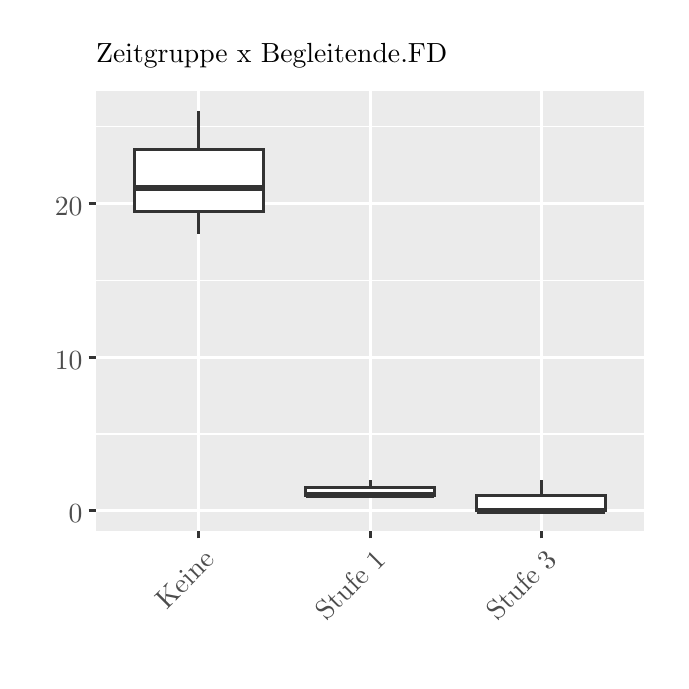
\begin{tikzpicture}[y=1mm, x=1mm, yscale=\globalscale,xscale=\globalscale, every node/.append style={scale=\globalscale}, inner sep=0pt, outer sep=0pt]
  \path[fill=white,line cap=round,line join=round,miter limit=10.0] ;



  \path[draw=white,fill=white,line cap=round,line join=round,line 
  width=0.38mm,miter limit=10.0] (-0.0, 80.0) rectangle (80.0, 0.0);



  \path[fill=cebebeb,line cap=round,line join=round,line width=0.38mm,miter 
  limit=10.0] (8.51, 72.09) rectangle (78.07, 16.31);



  \path[draw=white,line cap=butt,line join=round,line width=0.19mm,miter 
  limit=10.0] (8.51, 28.6) -- (78.07, 28.6);



  \path[draw=white,line cap=butt,line join=round,line width=0.19mm,miter 
  limit=10.0] (8.51, 48.1) -- (78.07, 48.1);



  \path[draw=white,line cap=butt,line join=round,line width=0.19mm,miter 
  limit=10.0] (8.51, 67.61) -- (78.07, 67.61);



  \path[draw=white,line cap=butt,line join=round,line width=0.38mm,miter 
  limit=10.0] (8.51, 18.85) -- (78.07, 18.85);



  \path[draw=white,line cap=butt,line join=round,line width=0.38mm,miter 
  limit=10.0] (8.51, 38.35) -- (78.07, 38.35);



  \path[draw=white,line cap=butt,line join=round,line width=0.38mm,miter 
  limit=10.0] (8.51, 57.86) -- (78.07, 57.86);



  \path[draw=white,line cap=butt,line join=round,line width=0.38mm,miter 
  limit=10.0] (21.55, 16.31) -- (21.55, 72.09);



  \path[draw=white,line cap=butt,line join=round,line width=0.38mm,miter 
  limit=10.0] (43.29, 16.31) -- (43.29, 72.09);



  \path[draw=white,line cap=butt,line join=round,line width=0.38mm,miter 
  limit=10.0] (65.03, 16.31) -- (65.03, 72.09);



  \path[draw=c333333,line cap=butt,line join=round,line width=0.38mm,miter 
  limit=10.0] (21.55, 64.68) -- (21.55, 69.56);



  \path[draw=c333333,line cap=butt,line join=round,line width=0.38mm,miter 
  limit=10.0] (21.55, 56.88) -- (21.55, 53.95);



  \path[draw=c333333,fill=white,line cap=butt,line join=miter,line 
  width=0.38mm,miter limit=10.0] (13.41, 64.68) -- (13.41, 56.88) -- (29.71, 
  56.88) -- (29.71, 64.68) -- (13.41, 64.68) -- (13.41, 64.68)-- cycle;



  \path[draw=c333333,line cap=butt,line join=miter,line width=0.75mm,miter 
  limit=10.0] (13.41, 59.81) -- (29.71, 59.81);



  \path[draw=c333333,line cap=butt,line join=round,line width=0.38mm,miter 
  limit=10.0] (43.29, 21.77) -- (43.29, 22.75);



  \path[draw=c333333,line cap=butt,line join=round,line width=0.38mm,miter 
  limit=10.0] ;



  \path[draw=c333333,fill=white,line cap=butt,line join=miter,line 
  width=0.38mm,miter limit=10.0] (35.14, 21.77) -- (35.14, 20.8) -- (51.44, 
  20.8) -- (51.44, 21.77) -- (35.14, 21.77) -- (35.14, 21.77)-- cycle;



  \path[draw=c333333,line cap=butt,line join=miter,line width=0.75mm,miter 
  limit=10.0] (35.14, 20.8) -- (51.44, 20.8);



  \path[draw=c333333,line cap=butt,line join=round,line width=0.38mm,miter 
  limit=10.0] (65.03, 20.8) -- (65.03, 22.75);



  \path[draw=c333333,line cap=butt,line join=round,line width=0.38mm,miter 
  limit=10.0] ;



  \path[draw=c333333,fill=white,line cap=butt,line join=miter,line 
  width=0.38mm,miter limit=10.0] (56.87, 20.8) -- (56.87, 18.85) -- (73.18, 
  18.85) -- (73.18, 20.8) -- (56.87, 20.8) -- (56.87, 20.8)-- cycle;



  \path[draw=c333333,line cap=butt,line join=miter,line width=0.75mm,miter 
  limit=10.0] (56.87, 18.85) -- (73.18, 18.85);



  \node[text=c4d4d4d,anchor=south east] (text5771) at (6.77, 17.33){0};



  \node[text=c4d4d4d,anchor=south east] (text8242) at (6.77, 36.84){10};



  \node[text=c4d4d4d,anchor=south east] (text7705) at (6.77, 56.35){20};



  \path[draw=c333333,line cap=butt,line join=round,line width=0.38mm,miter 
  limit=10.0] (7.55, 18.85) -- (8.51, 18.85);



  \path[draw=c333333,line cap=butt,line join=round,line width=0.38mm,miter 
  limit=10.0] (7.55, 38.35) -- (8.51, 38.35);



  \path[draw=c333333,line cap=butt,line join=round,line width=0.38mm,miter 
  limit=10.0] (7.55, 57.86) -- (8.51, 57.86);



  \path[draw=c333333,line cap=butt,line join=round,line width=0.38mm,miter 
  limit=10.0] (21.55, 15.34) -- (21.55, 16.31);



  \path[draw=c333333,line cap=butt,line join=round,line width=0.38mm,miter 
  limit=10.0] (43.29, 15.34) -- (43.29, 16.31);



  \path[draw=c333333,line cap=butt,line join=round,line width=0.38mm,miter 
  limit=10.0] (65.03, 15.34) -- (65.03, 16.31);



  \node[text=c4d4d4d,anchor=south east,cm={ 0.71,0.71,-0.71,0.71,(23.69, 
  -67.57)}] (text8905) at (0.0, 80.0){Keine};



  \node[text=c4d4d4d,anchor=south east,cm={ 0.71,0.71,-0.71,0.71,(45.43, 
  -67.57)}] (text2910) at (0.0, 80.0){Stufe 1};



  \node[text=c4d4d4d,anchor=south east,cm={ 0.71,0.71,-0.71,0.71,(67.16, 
  -67.57)}] (text6653) at (0.0, 80.0){Stufe 3};



  \node[anchor=south west] (text8784) at (8.51, 75.04){Zeitgruppe x 
  Begleitende.FD};




\end{tikzpicture}
